\scanpage{15}
\textcircled{7} Réconstruction des I-groupoïde fondamentaux $\Pi_1(\mathfrak X';J)$ de $\mathfrak X'$, et des opérations de $\mathcal G'$ dessus, en termes de l'extension $\unsure{\mathcal E|\Sigma}'$ de $\mathcal G'$ par $\pi_1$, et de l'opération de $\unsure{\mathcal E|\Sigma}'$ sur $\widetilde{\mathfrak X}'(J)$ et $\widetilde{\mathfrak X}'(J)\longrightarrow J$ [et des applications (7) (8)
\diagram{\begin{tikzcd}[ampersand replacement=\&]
\Psi^{\mathrm{ex}}:\widetilde{\mathfrak X}'(J) \arrow[r] \& \operatorname{Splitt}(\unsure{\mathcal E|\Sigma}'/\mathcal G')/\pi_1
\end{tikzcd}}
\diagram{\begin{tikzcd}[ampersand replacement=\&]
\Psi_{\unsure{j}}:\bigl(\widetilde{\mathfrak X}'(j) \arrow[r,dash] \& \operatorname{Splitt}(\unsure{\mathcal E|\Sigma}'_j/\mathcal G'_j)\bigr)].
\end{tikzcd}}
\margin{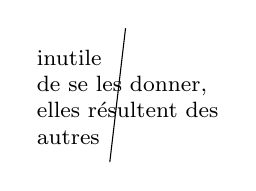
\begin{tikzpicture}[x=1cm,y=1cm]
\node[anchor=north west,align=left,font=\footnotesize] at (0,0) {inutile\\de se les donner,\\elles résultent des\\autres};
\draw (1.25,0.15) -- (1.05,-1.55);
\end{tikzpicture}}
\[
\operatorname{Ob}\Pi_1=J
\]
\deleted{\unsure{Soit} $j,j'\in J$}

\uline{NB} si $\widetilde\xi\in\widetilde{\mathfrak X}'(J)$, $\widetilde{\mathfrak X}'[j]$ (rev universel de $\mathfrak X'$ en $j$) s'identifie à $\widetilde{\mathfrak X}'$ (puisque $\widetilde\xi$ est un p\textsuperscript{t} marqué de $\widetilde{\mathfrak X}'$ au dessus de $j$
\diagram{\begin{tikzcd}[ampersand replacement=\&]
\widetilde{\mathfrak X}' \arrow[r,"\unsure{\varphi|\psi}_{\widetilde\xi}"] \& \widetilde{\mathfrak X}'[j]
\end{tikzcd}}
Si $\gamma\in\pi_1$, on aura
\[
\Psi_{\gamma\cdot\widetilde\xi}=\Psi_{\widetilde\xi}\circ\gamma_{\widetilde{\mathfrak X}'}^{\deleted{\unsure{-1}}}
\]
donc on peut dire, indépendamment du choix du p\textsuperscript{t} base $\widetilde\xi$
\diagram{\begin{tikzcd}[ampersand replacement=\&]
\widetilde{\mathfrak X}'[j] \& 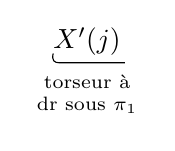
\begin{tikzpicture}[baseline=(torsorfactor.base),x=1cm,y=1cm]
\node[inner sep=0pt] (torsorfactor) at (0,0) {$\mathfrak X'(j)$};
\draw (-0.43,-0.15) .. controls (-0.45,-0.24) and (-0.42,-0.27) .. (-0.35,-0.27) -- (0.48,-0.27);
\node[anchor=north,align=center,font=\scriptsize] at (0,-0.30) {torseur à\\dr sous $\pi_1$};
\end{tikzpicture}\mathbin{\wedge}_{\pi_1}\widetilde{\mathfrak X}' \arrow[l,"\sim"']
\end{tikzcd}}
\mspage{14}
